% Document class
\documentclass{article}

% For figures
\usepackage{graphicx} % more modern
\usepackage{subfigure} 
% For citations
\usepackage{natbib}

% For algorithms
\usepackage{algorithm}
%\usepackage{algorithmic}

% As of 2011, we use the hyperref package to produce hyperlinks in the
% resulting PDF.  If this breaks your system, please commend out the
% following usepackage line and replace \usepackage{cs4437cs9637} with
% \usepackage[nohyperref]{cs4437cs9637} above.
\usepackage{hyperref}

% Packages hyperref and algorithmic misbehave sometimes.  We can fix
% this with the following command.
\newcommand{\theHalgorithm}{\arabic{algorithm}}

% Employ the following version of the ``usepackage'' statement for
% submitting the draft version of the paper for review.  This will set
% the note in the first column to ``Under review.  Do not distribute.''
\usepackage{cs4437cs9637} 

\begin{document}

% The \cstitle you define below is probably too long as a header.
% Therefore, a short form for the running title is supplied here:
\cstitlerunning{Project Proposal}

\twocolumn[
\cstitle{Evaluating Patterns in Critically Acclaimed Music}

% It is OKAY to include author information
\csauthor{Paul Bartlett (\normalsize\emph{\# 250753008})}{\href{mailto:pbartle7@uwo.ca}{\nolinkurl{pbartle7@uwo.ca}}}
\csaddress{The University Of Western Ontario}

% You may provide any keywords that you 
% find helpful for describing your paper; these are used to populate 
% the "keywords" metadata in the PDF but will not be shown in the document
\cskeywords{}

\vskip 0.3in
]

\begin{abstract} 
{\bf } The purpose of this analysis is to identify relationships between
musical genre of critically acclaimed albums and time. The dataset used
for this analysis contains over 18,000 reviews from Pitchfork from
January 5th, 1999 to January 8th, 2017. It contains important data
including release year, artist name, genre, and a score ranging from
0.0-10.0. The findings may be useful for determining what the most
successful genre of critically acclaimed music is for each of the last
18 years and what is going to be the most successful in the future. \end{abstract} 


\begin{verbatim}
## Warning: running command 'ls ../input' had status 127
\end{verbatim}

\section{Description of Applied
Problem}\label{description-of-applied-problem}

\subsection{Existing solutions to similar
problems}\label{existing-solutions-to-similar-problems}

The trends of popular music can easily be attained through the various
Billboard charts that have existed since 1955. A group of scientists
from the University of London analyzed around 17,000 songs that charted
on the U.S. Billboard Hot 100 over the last 50 years and created a
visualization of the popularity of musical genres over time
\citep{Billboard100}. The problem with getting data from these charts is
that popular music generally isn't critically acclaimed, and is
therefore not as interesting as data from sources that evaluate music
more objectively. Another source that uses visualization of this problem
well is musicmap \citep{musicmap}. The website contains information
about hundreds of genres of music and their history. It provides a great
overview of all the popular strands of music, but doesn't go into too
much depth about specific artists or albums. It does provide a good
overview of all genres regardless of popularity, but I'm more interested
in evaluating the history of genres from the best albums created by
artists.

\subsection{Pitchfork solution}\label{pitchfork-solution}

As various breakthroughs in music happen, there is generally a shift in
the type of genres that become popular. Artists get influenced by other
talented artists and adapt part of their style into their own music. In
addition, a good Pitchfork review can have a significant inpact on an
album's popularity. This is very important for independant artists
because they don't have the resources or backing of a large label to get
their name out there. Using a dataset that includes over 18,000 reviews
from Pitchfork, I will be going through the data to find how critically
acclaimed music has changed over time. In addition, I will be looking
into applications of machine learning for predicting an album's score to
find out what influences this.

\section{Description of Available
Data}\label{description-of-available-data}

\subsection{Pitchfork}\label{pitchfork}

The dataset that I will be using is taken from Pitchfork. Pitchfork is
an online magazine that focuses on reviewing both popular and
independent music. It is one of the most popular platforms for users
interested in finding higher quality music. The data set for Pitchfork
Reviews from January 5th, 1999 to January 8th, 2017 is available on
kaggle \citep{kaggle}. There are 18,393 reviews that include important
data including release year, artist name, genre, and a score ranging
from 0.0-10.0. Considering that Pitchfork is one of the longest running
online review sites, it makes it a primary choice for useful data. There
may be some bias in review scores, notably staff preference, but
Pitchfork does cover a lot of genres with ratings similar to many other
music review platforms. Through looking at 18 years of data, we should
be able to find some notable trends.

\section{Analysis and Visualization}\label{analysis-and-visualization}

\subsection{Genre}\label{genre}

To analyze this data properly, we must use a method to take out only the
best reviews from the dataset. Fortunately, Pitchfork has a system to
distinguish the best albums called ``Best New Music''. Albums that
receive this tag are guaranteed to be of higher quality and therefore
valid for our analysis. Unfortunately, this feature launched in 2003 so
using it would leave out all the music before it was launched. By
looking at the data, we will be able to find the typical rating for an
album that gets the ``Best New Music'' tag and use that rating to take
all albums from the data set that are higher than the threshold. From
this, we should be able to classify each album that meets the
requirement by year and genre so that it can be used for visualization.

\subsubsection{Visualization}\label{visualization}

For visualization, I would like to do something similar to what was done
for visualizing the U.S. Billboard Hot 100 over the last 50 years
\citep{BillboardFigure}. The chart features spindles for each genre that
run vertically with the width of the spindles proportional to the
frequency of the genre. The y-axis contains the year so the viewer can
easily compare between each year to see what genre is the most popular
or the least popular. Since I do not have much experience with
visualization, it is possible that doing something similar will be too
difficult to achieve. A simple way to visualize this in a similar way
would be to use a line graph, with each line representing a genre, the
x-axis covering each year, and the y-axis covering the frequency.

\subsection{Release}\label{release}

\subsubsection{Analysis}\label{analysis}

To analyze what release number is considered to be the best critically,
we will have to query all artists that have multiple releases on the
site. A similar analysis and visualization was done on kaggle by the
author of the data \citep{kaggleFirst}. The author only covered the
first and last album, but did complete an analysis on the number of
reviews for each artist. After this, we need to get the review scores of
each album from each of the artists with multiple releases. There might
be some bias in how release numbers are scored, mainly that a poor
release could potentially prevent the staff from Pitchfork from
reviewing later releases.

\subsubsection{Visualization}\label{visualization-1}

A Box plot would be perfectly suited for this data. Being able to
visualize the entire range of score for the releases while also seeing
the median and upper and lower quartiles is highly beneficial. There
would be a separate box plot for each release number up to the maximum
reviewed releases by an artist.

\newpage

\newpage

\begin{figure}
\centering
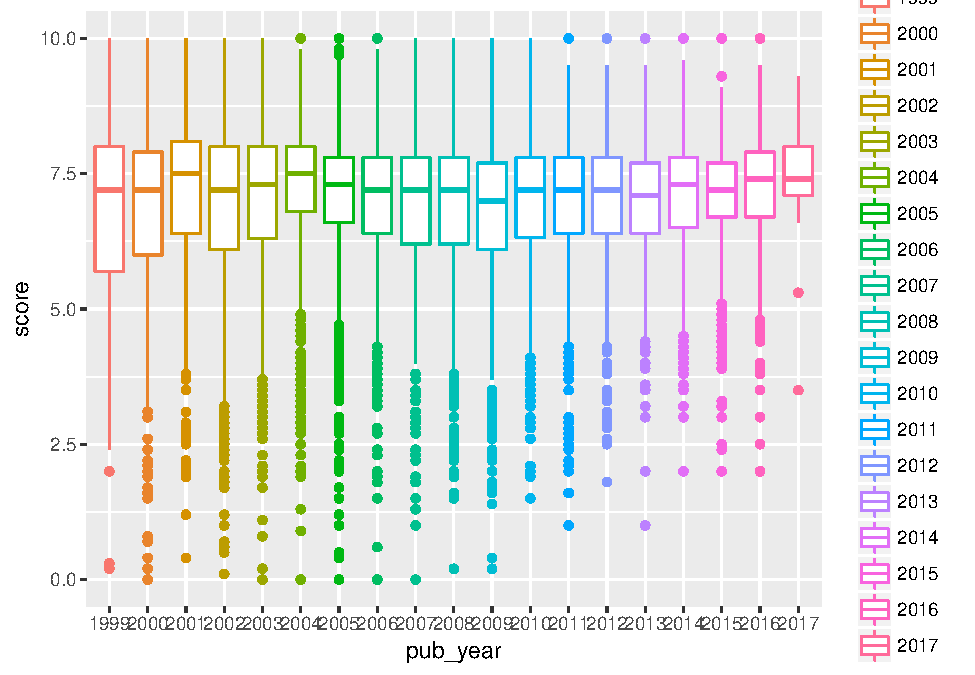
\includegraphics{report_files/figure-latex/score_year.pdf}
\caption{Boxplots of score by year \label{fig1}}
\end{figure}

\newpage

\newpage

\begin{figure}
\centering
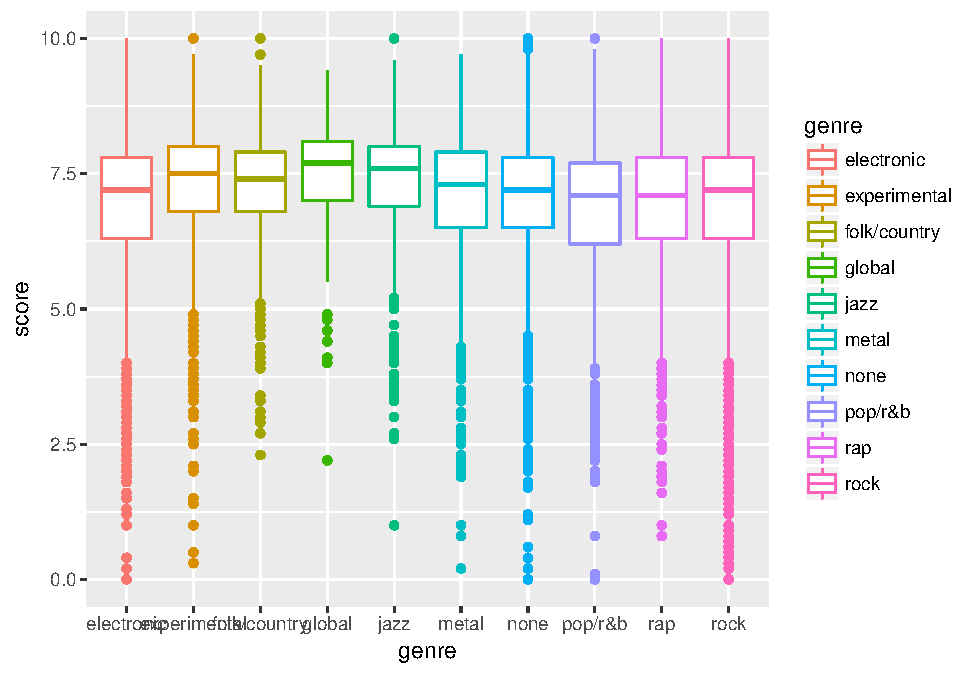
\includegraphics{report_files/figure-latex/score_genre.pdf}
\caption{Boxplots of score by genre \label{fig2}}
\end{figure}

\newpage

\begin{figure}
\centering
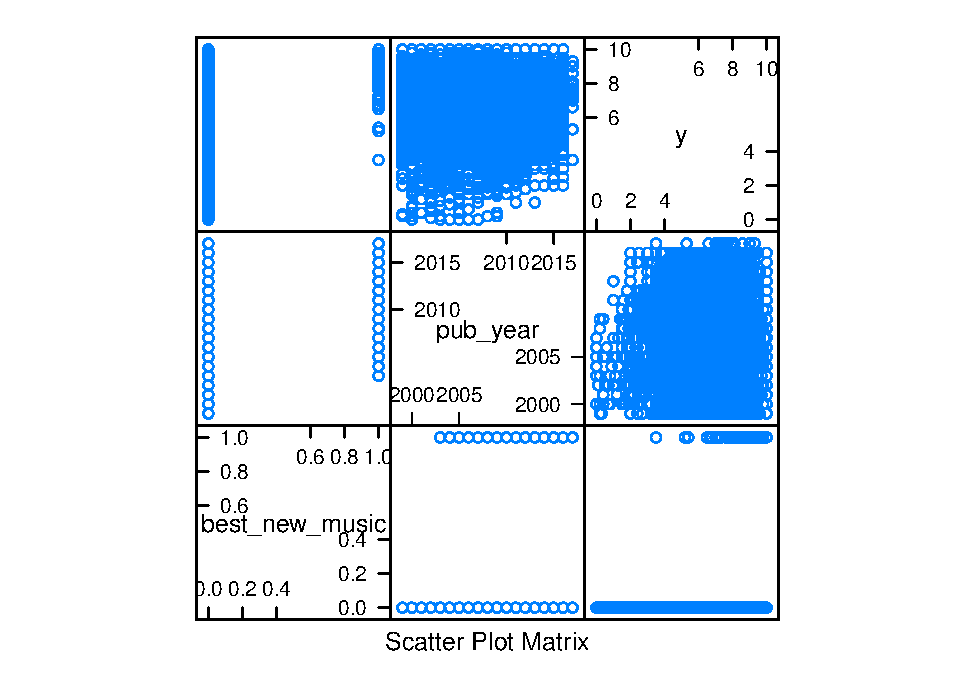
\includegraphics{report_files/figure-latex/scatterplot_matrix.pdf}
\caption{Scatterplot matrix of features \label{fig3}}
\end{figure}

\newpage

\bibliography{bibliography.bib}
\bibliographystyle{plainnat}

\end{document} 
